% Options for packages loaded elsewhere
\PassOptionsToPackage{unicode}{hyperref}
\PassOptionsToPackage{hyphens}{url}
%
\documentclass[
]{article}
\usepackage{amsmath,amssymb}
\usepackage{iftex}
\ifPDFTeX
  \usepackage[T1]{fontenc}
  \usepackage[utf8]{inputenc}
  \usepackage{textcomp} % provide euro and other symbols
\else % if luatex or xetex
  \usepackage{unicode-math} % this also loads fontspec
  \defaultfontfeatures{Scale=MatchLowercase}
  \defaultfontfeatures[\rmfamily]{Ligatures=TeX,Scale=1}
\fi
\usepackage{lmodern}
\ifPDFTeX\else
  % xetex/luatex font selection
\fi
% Use upquote if available, for straight quotes in verbatim environments
\IfFileExists{upquote.sty}{\usepackage{upquote}}{}
\IfFileExists{microtype.sty}{% use microtype if available
  \usepackage[]{microtype}
  \UseMicrotypeSet[protrusion]{basicmath} % disable protrusion for tt fonts
}{}
\makeatletter
\@ifundefined{KOMAClassName}{% if non-KOMA class
  \IfFileExists{parskip.sty}{%
    \usepackage{parskip}
  }{% else
    \setlength{\parindent}{0pt}
    \setlength{\parskip}{6pt plus 2pt minus 1pt}}
}{% if KOMA class
  \KOMAoptions{parskip=half}}
\makeatother
\usepackage{xcolor}
\usepackage[margin=1in]{geometry}
\usepackage{color}
\usepackage{fancyvrb}
\newcommand{\VerbBar}{|}
\newcommand{\VERB}{\Verb[commandchars=\\\{\}]}
\DefineVerbatimEnvironment{Highlighting}{Verbatim}{commandchars=\\\{\}}
% Add ',fontsize=\small' for more characters per line
\usepackage{framed}
\definecolor{shadecolor}{RGB}{248,248,248}
\newenvironment{Shaded}{\begin{snugshade}}{\end{snugshade}}
\newcommand{\AlertTok}[1]{\textcolor[rgb]{0.94,0.16,0.16}{#1}}
\newcommand{\AnnotationTok}[1]{\textcolor[rgb]{0.56,0.35,0.01}{\textbf{\textit{#1}}}}
\newcommand{\AttributeTok}[1]{\textcolor[rgb]{0.13,0.29,0.53}{#1}}
\newcommand{\BaseNTok}[1]{\textcolor[rgb]{0.00,0.00,0.81}{#1}}
\newcommand{\BuiltInTok}[1]{#1}
\newcommand{\CharTok}[1]{\textcolor[rgb]{0.31,0.60,0.02}{#1}}
\newcommand{\CommentTok}[1]{\textcolor[rgb]{0.56,0.35,0.01}{\textit{#1}}}
\newcommand{\CommentVarTok}[1]{\textcolor[rgb]{0.56,0.35,0.01}{\textbf{\textit{#1}}}}
\newcommand{\ConstantTok}[1]{\textcolor[rgb]{0.56,0.35,0.01}{#1}}
\newcommand{\ControlFlowTok}[1]{\textcolor[rgb]{0.13,0.29,0.53}{\textbf{#1}}}
\newcommand{\DataTypeTok}[1]{\textcolor[rgb]{0.13,0.29,0.53}{#1}}
\newcommand{\DecValTok}[1]{\textcolor[rgb]{0.00,0.00,0.81}{#1}}
\newcommand{\DocumentationTok}[1]{\textcolor[rgb]{0.56,0.35,0.01}{\textbf{\textit{#1}}}}
\newcommand{\ErrorTok}[1]{\textcolor[rgb]{0.64,0.00,0.00}{\textbf{#1}}}
\newcommand{\ExtensionTok}[1]{#1}
\newcommand{\FloatTok}[1]{\textcolor[rgb]{0.00,0.00,0.81}{#1}}
\newcommand{\FunctionTok}[1]{\textcolor[rgb]{0.13,0.29,0.53}{\textbf{#1}}}
\newcommand{\ImportTok}[1]{#1}
\newcommand{\InformationTok}[1]{\textcolor[rgb]{0.56,0.35,0.01}{\textbf{\textit{#1}}}}
\newcommand{\KeywordTok}[1]{\textcolor[rgb]{0.13,0.29,0.53}{\textbf{#1}}}
\newcommand{\NormalTok}[1]{#1}
\newcommand{\OperatorTok}[1]{\textcolor[rgb]{0.81,0.36,0.00}{\textbf{#1}}}
\newcommand{\OtherTok}[1]{\textcolor[rgb]{0.56,0.35,0.01}{#1}}
\newcommand{\PreprocessorTok}[1]{\textcolor[rgb]{0.56,0.35,0.01}{\textit{#1}}}
\newcommand{\RegionMarkerTok}[1]{#1}
\newcommand{\SpecialCharTok}[1]{\textcolor[rgb]{0.81,0.36,0.00}{\textbf{#1}}}
\newcommand{\SpecialStringTok}[1]{\textcolor[rgb]{0.31,0.60,0.02}{#1}}
\newcommand{\StringTok}[1]{\textcolor[rgb]{0.31,0.60,0.02}{#1}}
\newcommand{\VariableTok}[1]{\textcolor[rgb]{0.00,0.00,0.00}{#1}}
\newcommand{\VerbatimStringTok}[1]{\textcolor[rgb]{0.31,0.60,0.02}{#1}}
\newcommand{\WarningTok}[1]{\textcolor[rgb]{0.56,0.35,0.01}{\textbf{\textit{#1}}}}
\usepackage{graphicx}
\makeatletter
\newsavebox\pandoc@box
\newcommand*\pandocbounded[1]{% scales image to fit in text height/width
  \sbox\pandoc@box{#1}%
  \Gscale@div\@tempa{\textheight}{\dimexpr\ht\pandoc@box+\dp\pandoc@box\relax}%
  \Gscale@div\@tempb{\linewidth}{\wd\pandoc@box}%
  \ifdim\@tempb\p@<\@tempa\p@\let\@tempa\@tempb\fi% select the smaller of both
  \ifdim\@tempa\p@<\p@\scalebox{\@tempa}{\usebox\pandoc@box}%
  \else\usebox{\pandoc@box}%
  \fi%
}
% Set default figure placement to htbp
\def\fps@figure{htbp}
\makeatother
\setlength{\emergencystretch}{3em} % prevent overfull lines
\providecommand{\tightlist}{%
  \setlength{\itemsep}{0pt}\setlength{\parskip}{0pt}}
\setcounter{secnumdepth}{-\maxdimen} % remove section numbering
\usepackage{bookmark}
\IfFileExists{xurl.sty}{\usepackage{xurl}}{} % add URL line breaks if available
\urlstyle{same}
\hypersetup{
  pdftitle={Template},
  pdfauthor={Studentnames and studentnumbers here},
  hidelinks,
  pdfcreator={LaTeX via pandoc}}

\title{Template}
\author{Studentnames and studentnumbers here}
\date{2025-06-12}

\begin{document}
\maketitle

\section{Set-up your environment}\label{set-up-your-environment}

\begin{Shaded}
\begin{Highlighting}[]
\FunctionTok{require}\NormalTok{(tidyverse)}
\end{Highlighting}
\end{Shaded}

\begin{verbatim}
## Loading required package: tidyverse
\end{verbatim}

\begin{verbatim}
## -- Attaching core tidyverse packages ------------------------ tidyverse 2.0.0 --
## v dplyr     1.1.4     v readr     2.1.5
## v forcats   1.0.0     v stringr   1.5.1
## v ggplot2   3.5.2     v tibble    3.3.0
## v lubridate 1.9.4     v tidyr     1.3.1
## v purrr     1.0.4     
## -- Conflicts ------------------------------------------ tidyverse_conflicts() --
## x dplyr::filter() masks stats::filter()
## x dplyr::lag()    masks stats::lag()
## i Use the conflicted package (<http://conflicted.r-lib.org/>) to force all conflicts to become errors
\end{verbatim}

\section{Title Page}\label{title-page}

Include your names

Include the tutorial group number

Include your tutorial lecturer's name

\section{Part 1 - Identify a Social
Problem}\label{part-1---identify-a-social-problem}

Use APA referencing throughout your document.
\href{https://www.mendeley.com/guides/apa-citation-guide/}{Here's a link
to some explanation.}

\subsection{1.1 Describe the Social
Problem}\label{describe-the-social-problem}

Include the following:

\begin{itemize}
\item
  Why is this relevant?
\item
  \ldots{}
\end{itemize}

\section{Part 2 - Data Sourcing}\label{part-2---data-sourcing}

\subsection{2.1 Load in the data}\label{load-in-the-data}

Preferably from a URL, but if not, make sure to download the data and
store it in a shared location that you can load the data in from. Do not
store the data in a folder you include in the Github repository!

\begin{Shaded}
\begin{Highlighting}[]
\NormalTok{dataset }\OtherTok{\textless{}{-}}\NormalTok{ midwest}
\end{Highlighting}
\end{Shaded}

midwest is an example dataset included in the tidyverse package

\subsection{2.2 Provide a short summary of the
dataset(s)}\label{provide-a-short-summary-of-the-datasets}

\begin{Shaded}
\begin{Highlighting}[]
\FunctionTok{head}\NormalTok{(dataset)}
\end{Highlighting}
\end{Shaded}

\begin{verbatim}
## # A tibble: 6 x 28
##     PID county   state  area poptotal popdensity popwhite popblack popamerindian
##   <int> <chr>    <chr> <dbl>    <int>      <dbl>    <int>    <int>         <int>
## 1   561 ADAMS    IL    0.052    66090      1271.    63917     1702            98
## 2   562 ALEXAND~ IL    0.014    10626       759      7054     3496            19
## 3   563 BOND     IL    0.022    14991       681.    14477      429            35
## 4   564 BOONE    IL    0.017    30806      1812.    29344      127            46
## 5   565 BROWN    IL    0.018     5836       324.     5264      547            14
## 6   566 BUREAU   IL    0.05     35688       714.    35157       50            65
## # i 19 more variables: popasian <int>, popother <int>, percwhite <dbl>,
## #   percblack <dbl>, percamerindan <dbl>, percasian <dbl>, percother <dbl>,
## #   popadults <int>, perchsd <dbl>, percollege <dbl>, percprof <dbl>,
## #   poppovertyknown <int>, percpovertyknown <dbl>, percbelowpoverty <dbl>,
## #   percchildbelowpovert <dbl>, percadultpoverty <dbl>,
## #   percelderlypoverty <dbl>, inmetro <int>, category <chr>
\end{verbatim}

In this case we see 28 variables, but we miss some information on what
units they are in. We also don't know anything about the year/moment in
which this data has been captured.

\begin{Shaded}
\begin{Highlighting}[]
\NormalTok{inline\_code }\OtherTok{=} \ConstantTok{TRUE}
\end{Highlighting}
\end{Shaded}

These are things that are usually included in the metadata of the
dataset. For your project, you need to provide us with the information
from your metadata that we need to understand your dataset of choice.

\subsection{2.3 Describe the type of variables
included}\label{describe-the-type-of-variables-included}

Think of things like:

\begin{itemize}
\item
  Do the variables contain health information or SES information?
\item
  Have they been measured by interviewing individuals or is the data
  coming from administrative sources?
\end{itemize}

\emph{For the sake of this example, I will continue with the
assignment\ldots{}}

\section{Part 3 - Quantifying}\label{part-3---quantifying}

\subsection{3.1 Data cleaning}\label{data-cleaning}

Say we want to include only larger distances (above 2) in our dataset,
we can filter for this.

\begin{Shaded}
\begin{Highlighting}[]
\FunctionTok{mean}\NormalTok{(dataset}\SpecialCharTok{$}\NormalTok{percollege)}
\end{Highlighting}
\end{Shaded}

\begin{verbatim}
## [1] 18.27274
\end{verbatim}

Please use a separate `R block' of code for each type of cleaning. So,
e.g.~one for missing values, a new one for removing unnecessary
variables etc.

\subsection{3.2 Generate necessary
variables}\label{generate-necessary-variables}

Variable 1

Variable 2

\subsection{3.3 Visualize temporal
variation}\label{visualize-temporal-variation}

\subsection{3.4 Visualize spatial
variation}\label{visualize-spatial-variation}

Here you provide a description of why the plot above is relevant to your
specific social problem.

\subsection{3.5 Visualize sub-population
variation}\label{visualize-sub-population-variation}

What is the poverty rate by state?

\begin{Shaded}
\begin{Highlighting}[]
\NormalTok{dataset}\SpecialCharTok{$}\NormalTok{inmetro }\OtherTok{\textless{}{-}}\NormalTok{ dataset}\SpecialCharTok{$}\NormalTok{inmetro }\SpecialCharTok{\%\textgreater{}\%} \FunctionTok{as.factor}\NormalTok{()}
\CommentTok{\# Boxplot of poverty rate by state using the \textquotesingle{}midwest\textquotesingle{} dataset}
\FunctionTok{ggplot}\NormalTok{(dataset, }\FunctionTok{aes}\NormalTok{(}\AttributeTok{x =}\NormalTok{ inmetro, }\AttributeTok{y =}\NormalTok{ percadultpoverty)) }\SpecialCharTok{+}
  \FunctionTok{geom\_boxplot}\NormalTok{() }\SpecialCharTok{+}
  \FunctionTok{labs}\NormalTok{(}
    \AttributeTok{title =} \StringTok{"Distribution of Poverty Rates by Metropolitan status (Midwest counties)"}\NormalTok{,}
    \AttributeTok{x =} \StringTok{"Metropolitan Area"}\NormalTok{,}
    \AttributeTok{y =} \StringTok{"Poverty Rate of Adults (\%)"}
\NormalTok{  ) }\SpecialCharTok{+}
  \FunctionTok{theme\_minimal}\NormalTok{() }\SpecialCharTok{+}
  \FunctionTok{theme}\NormalTok{(}
    \AttributeTok{legend.position =} \StringTok{"right"}
\NormalTok{  )}
\end{Highlighting}
\end{Shaded}

\pandocbounded{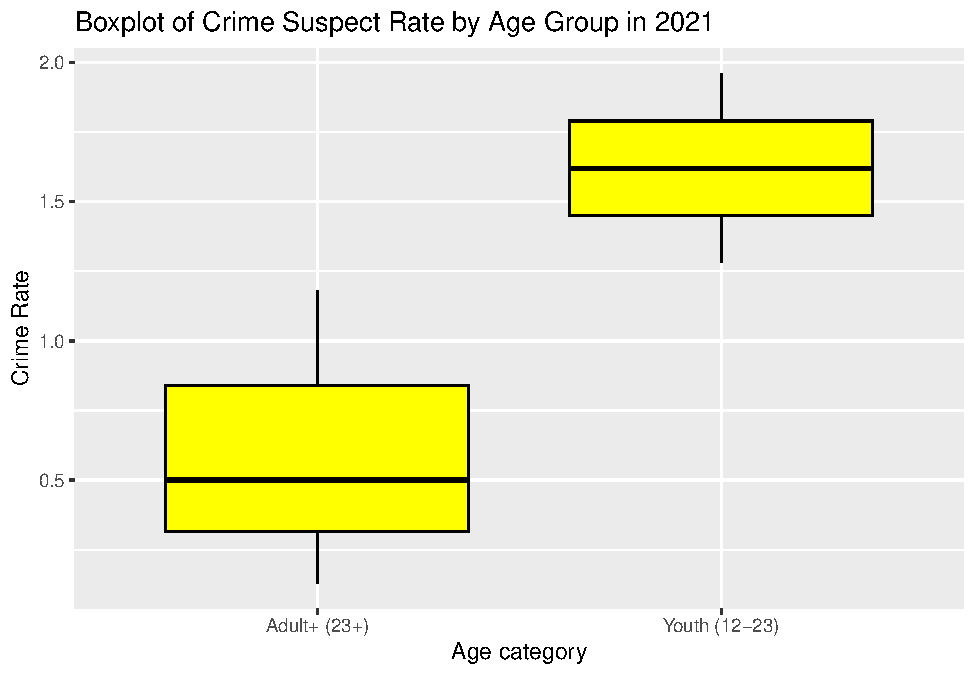
\includegraphics[keepaspectratio]{Template_Assignment_files/figure-latex/visualise_subpopulations-1.pdf}}

Here you provide a description of why the plot above is relevant to your
specific social problem.

\subsection{3.6 Event analysis}\label{event-analysis}

Analyze the relationship between two variables.

Here you provide a description of why the plot above is relevant to your
specific social problem.

\section{Part 4 - Discussion}\label{part-4---discussion}

\subsection{4.1 Discuss your findings}\label{discuss-your-findings}

\section{Part 5 - Reproducibility}\label{part-5---reproducibility}

\subsection{5.1 Github repository link}\label{github-repository-link}

Provide the link to your PUBLIC repository here: \ldots{}

\subsection{5.2 Reference list}\label{reference-list}

Use APA referencing throughout your document.

\end{document}
